\section{Antenna Design 1 - Monopole}

\begin{figure}[htbp]
    \begin{subfigure}[b]{0.49\linewidth}
        \centering
        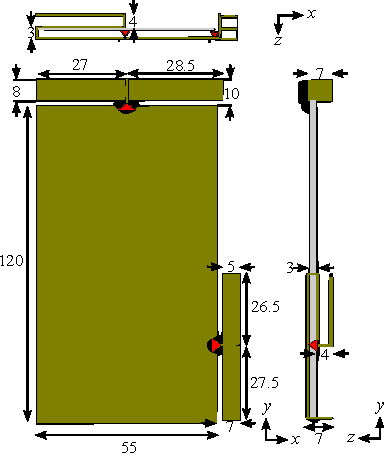
\includegraphics{img/tech_sol/monopole/tech_drawing}
        \caption{Technical drawing.}
        \label{fig:ant1technical}
    \end{subfigure}
    \hfill
    \begin{subfigure}[b]{0.49\linewidth}
        \centering
        \includegraphics{img/tech_sol/schematic_tuning_1}
        \caption{Tuning/matching circuit.}
        \label{fig:ant1schematic}
    \end{subfigure}
    \caption{Technical drawing and tuning circuit for the antenna.  The antennas are built on FR-4 board using \SI{35}{\micro\meter} copper. There is a matching circuit as shown for each of the two feeds.}
    \label{fig:ant2techschem}
\end{figure}

The component values of the matching circuit for both the bottom and side antenna are provided in table \ref{}

\begin{table}[]
\centering
\begin{tabular}{|l|l|l|}
\hline
      & C1    & L1    \\ \hline
Ant 1 & 3.017 & 7.996 \\ \hline
Ant 2 & 1.807 & 5.265 \\ \hline
\end{tabular}
\caption{Matching circuit}
\label{tab:ant1_matching}
\end{table}

\begin{itemize}
\item Antenna 1 
\begin{itemize}
\item C1 $3.01734$
\item I $7.99632$
\end{itemize}
\item Antenna 2
\begin{itemize}
\item C1 $1.80676$
\item I $5.26483$
\end{itemize}



